\usetikzlibrary{shapes,snakes}

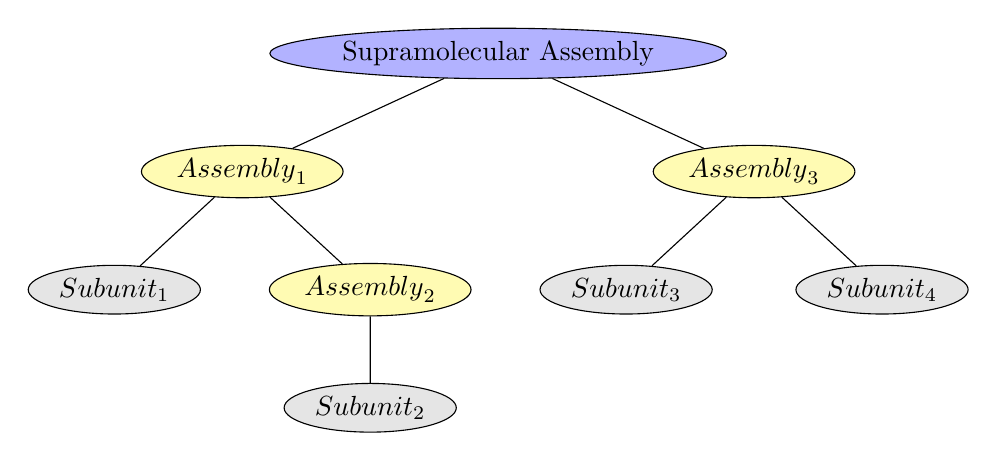
\begin{tikzpicture}[
every node/.style={inner sep=2pt},
level/.style={sibling distance=65mm/#1},
root/.append style={ellipse,draw,fill=blue!30},
symm/.append style={ellipse,draw,fill=yellow!30},
 pdb/.append style={ellipse,draw,fill=black!10},
 ]
\node [root](rt){Supramolecular Assembly}
	child{node[symm](s1){$\text{Assembly}_1$}
		child{node[pdb](p1){$\text{Subunit}_1$}}
		child{node[symm](s2){$\text{Assembly}_2$}
			child{node[pdb](p2){$\text{Subunit}_2$}}
		}
	}
	child{node[symm](s3){$\text{Assembly}_3$}
		child{node[pdb](p3){$\text{Subunit}_3$}}
		child{node[pdb](p4){$\text{Subunit}_4$}}
	}
;
\path (s1) -- (s3) node [scale=3,midway] {$\hdots$};
\path (p3) -- (p4) node [scale=1.5,midway] {$\hdots$};
\path (p1) -- (s2) node [scale=1.5,midway] {$\hdots$};
\end{tikzpicture}
